\documentclass[11pt]{article}

%--------------------------------------------------
% Packages
%--------------------------------------------------
\usepackage[margin=1in]{geometry}
\usepackage{amsmath,amssymb}
\usepackage{graphicx}
\usepackage{hyperref}
\usepackage{booktabs}
\usepackage{enumitem}
\usepackage{xcolor}
\usepackage{titlesec}
\usepackage{tikz}
\usetikzlibrary{shapes.geometric, arrows.meta, positioning, fit, backgrounds}
\usepackage{fancyhdr}
\usepackage{microtype}
\usepackage{parskip}
\usepackage{tcolorbox}
\tcbuselibrary{skins, breakable}
\usepackage{listings}
\usepackage{float}

%--------------------------------------------------
% Colors
%--------------------------------------------------
\definecolor{primary}{RGB}{0,74,148}
\definecolor{accent}{RGB}{220,50,47}
\definecolor{lightgray}{RGB}{245,245,245}
\definecolor{darkgray}{RGB}{80,80,80}
\definecolor{plannerblue}{RGB}{173,216,230}
\definecolor{toolgreen}{RGB}{144,238,144}
\definecolor{llmpurple}{RGB}{216,191,216}
\definecolor{memoryorange}{RGB}{255,228,181}
\definecolor{codebg}{RGB}{248,248,248}

%--------------------------------------------------
% Section formatting
%--------------------------------------------------
\titleformat{\section}{\large\bfseries\color{primary}}{}{0em}{}[\vspace{-0.5em}\rule{\linewidth}{0.4pt}]
\titleformat{\subsection}{\normalsize\bfseries\color{darkgray}}{}{0em}{}

%--------------------------------------------------
% Header / Footer
%--------------------------------------------------
\pagestyle{fancy}
\fancyhf{}
\rhead{\small\color{darkgray} ESE 561 --- Final Project Report}
\lhead{\small\color{darkgray} SAGE: Self-Adaptive Goal-directed Executor}
\cfoot{\thepage}
\renewcommand{\headrulewidth}{0.4pt}

%--------------------------------------------------
% Hyperref setup
%--------------------------------------------------
\hypersetup{
  colorlinks=true,
  linkcolor=primary,
  urlcolor=primary,
  citecolor=primary
}

%--------------------------------------------------
% TColorBox styles
%--------------------------------------------------
\tcbset{
  boxstyle/.style={
    enhanced, breakable,
    colback=lightgray,
    colframe=primary,
    fonttitle=\bfseries,
    boxrule=0.6pt,
    arc=3pt,
    left=6pt, right=6pt, top=4pt, bottom=4pt
  }
}

%--------------------------------------------------
% Code listing style
%--------------------------------------------------
\lstset{
  backgroundcolor=\color{codebg},
  basicstyle=\ttfamily\small,
  breaklines=true,
  frame=single,
  rulecolor=\color{lightgray},
  numbers=left,
  numberstyle=\tiny\color{gray},
  keywordstyle=\color{primary}\bfseries,
  commentstyle=\color{gray}\itshape,
  stringstyle=\color{accent},
  showstringspaces=false,
  tabsize=2,
}

%==================================================
\begin{document}
%==================================================

%--------------------------------------------------
% Title block
%--------------------------------------------------
\begin{center}
  {\LARGE\bfseries\color{primary} SAGE: Self-Adaptive Goal-directed Executor}\\[4pt]
  {\large A Multi-Tool LLM Agent with Hierarchical Planning\\
  and Evidence-Guided Reasoning}\\[10pt]
  \rule{\linewidth}{1pt}\\[6pt]
  {\normalsize
  \textbf{Course:} ESE 561 --- Artificial Intelligence \hspace{1.5cm}
  \textbf{Date:} April 2026 \\[4pt]
  \textbf{Team Members:} Shams Rupak \quad $\cdot$ \quad Gagan Sapkota \\[4pt]
  \textbf{Stony Brook University} \hspace{1.8cm} \textbf{Team Size:} 2
  }\\[4pt]
  \rule{\linewidth}{0.4pt}
\end{center}

\vspace{0.4em}

%--------------------------------------------------
\section{Abstract}
%--------------------------------------------------

We present SAGE (Self-Adaptive Goal-directed Executor), a multi-tool LLM-based agent for automated research synthesis. Given a complex, open-ended research question, SAGE decomposes it into a Directed Acyclic Graph (DAG) of sub-goals using a deterministic Python planner, executes each sub-goal through a ReAct-style reasoning loop with real tools (web search, URL fetching, claim extraction, code execution, cross-referencing), evaluates the gathered evidence through an independent Evidence Critic module, and adaptively re-plans when evidence is insufficient or contradictory. The system produces a structured, citation-aware analytical report with per-claim provenance tracking.

The central design principle of SAGE is the explicit separation of planning logic from neural reasoning: all high-level decision-making---goal decomposition, execution scheduling, stopping conditions, and adaptive re-planning---is implemented as deterministic Python code external to the LLM. The LLM is scoped strictly to per-step reasoning and tool proposal within individual sub-goals. This architectural boundary makes the system transparent, auditable, and empirically interrogable.

We evaluate SAGE through an ablation study comparing three conditions: full SAGE (DAG planner + ReAct + Evidence Critic), flat ReAct (no planner or critic), and a single LLM call baseline. Results demonstrate that the planning and critique layers consistently improve output structure, source grounding, and self-correction behavior across diverse research queries.

%--------------------------------------------------
\section{Introduction and Motivation}
%--------------------------------------------------

Large language models have demonstrated remarkable capability in isolated reasoning tasks, yet they remain fundamentally reactive: given a prompt, they produce an output. This single-call paradigm collapses under complex, multi-faceted queries that require sustained goal-directed behavior, tool interaction, self-correction, and adaptive re-planning.

Consider the task: \textit{``Analyze the trade-offs between transformer-based and recurrent architectures for long-context reasoning, citing empirical evidence and identifying open research questions.''} A single LLM call yields a plausible but unverifiable response. A proper answer requires decomposing the question into sub-goals, actively searching for evidence, evaluating source reliability, reconciling contradictions across sources, and synthesizing findings with tracked provenance.

SAGE is designed to tackle exactly this class of problem. The agent performs \emph{deep research synthesis}: given a complex research query, it autonomously plans a multi-step investigation, gathers evidence from external tools, evaluates and critiques that evidence, and produces a structured, citation-aware synthesis.

This project is motivated by a central question that runs through the course: \textit{Where does the intelligence of an LLM-based system come from---the neural model, or the surrounding structure?} SAGE is designed to make that boundary explicit and empirically interrogable. By implementing all planning logic as deterministic code and scoping the LLM to per-step reasoning, we can directly measure the contribution of each layer through ablation.

\subsection{Design Goals}

SAGE was designed with four explicit goals:

\textbf{Transparency.} Every planning decision---which sub-goal to pursue, when to retry, when to re-plan---is made by auditable Python code, not by opaque LLM reasoning. This makes the system's behavior predictable and debuggable.

\textbf{Self-Correction.} The Evidence Critic creates a feedback loop that catches low-quality evidence, contradictions, and insufficient coverage before they propagate to the final synthesis. This is the mechanism that distinguishes SAGE from a fixed pipeline.

\textbf{Grounded Output.} Every claim in the final report is traceable to a specific tool call and source URL through the provenance system. This directly addresses the hallucination problem inherent in ungrounded LLM outputs.

\textbf{Empirical Interrogability.} The ablation study framework allows us to quantitatively measure the contribution of each architectural layer, connecting system design to the course's theoretical themes about the sources of intelligence in AI systems.

%--------------------------------------------------
\section{Related Work}
%--------------------------------------------------

SAGE draws on several lines of work in LLM-based agent design:

\textbf{ReAct.} Yao et al.\ introduced the ReAct paradigm, which interleaves reasoning traces with tool actions, grounding LLM outputs in external observations. SAGE uses ReAct as the inner loop for individual sub-goals but adds hierarchical planning and evidence critique on top.

\textbf{Plan-and-Execute Agents.} Wang et al.\ demonstrated that separating planning from execution improves agent reliability on multi-step tasks. SAGE extends this with a DAG-based planner that supports dependency tracking, priority scheduling, and adaptive re-planning.

\textbf{Self-Reflection and Critique.} Shinn et al.\ (Reflexion) showed that LLM agents benefit from self-evaluation loops. SAGE's Evidence Critic module implements a structured version of this idea, with fixed JSON schemas and deterministic override rules that prevent infinite retry loops.

\textbf{Tool-Augmented LLMs.} Schick et al.\ (Toolformer) and subsequent work demonstrated that LLMs can effectively use external tools when given appropriate interfaces. SAGE implements a clean tool registry with five tools, each returning standardized result dictionaries.

The key distinction of SAGE from prior work is the \emph{explicit architectural separation} of planning, reasoning, and critique into distinct modules with well-defined interfaces. This is not merely an engineering choice---it is the central design principle that enables the ablation study and connects the system to the course's themes about neuro-symbolic integration.

%--------------------------------------------------
\section{System Design}
%--------------------------------------------------

SAGE decomposes the agent into five explicit layers, as shown in Figure~\ref{fig:arch}. Each layer has a defined interface, ensuring that planning logic and LLM reasoning remain clearly separated.

\begin{figure}[H]
\centering
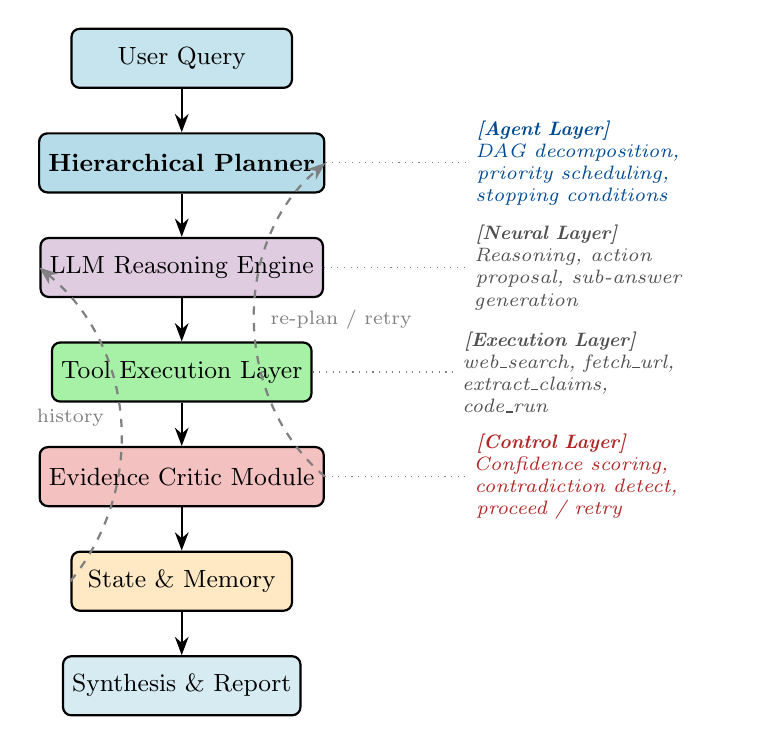
\begin{tikzpicture}[
  node distance=0.55cm and 0.4cm,
  every node/.style={font=\small},
  block/.style={rectangle, rounded corners=3pt, minimum width=2.8cm,
                minimum height=0.75cm, text centered, draw, thick},
  arrow/.style={-Stealth, thick},
  dasharrow/.style={-Stealth, thick, dashed, color=gray}
]

%--- Layers ---%
\node[block, fill=plannerblue!70]  (input)    {User Query};
\node[block, fill=plannerblue!90,  below=of input]  (planner)  {\textbf{Hierarchical Planner}};
\node[block, fill=llmpurple!80,    below=of planner] (llm)     {LLM Reasoning Engine};
\node[block, fill=toolgreen!80,    below=of llm]    (tools)    {Tool Execution Layer};
\node[block, fill=accent!30,       below=of tools]  (critic)   {Evidence Critic Module};
\node[block, fill=memoryorange!80, below=of critic] (memory)   {State \& Memory};
\node[block, fill=plannerblue!50,  below=of memory] (synth)    {Synthesis \& Report};

%--- Arrows (main flow) ---%
\draw[arrow] (input)   -- (planner);
\draw[arrow] (planner) -- (llm);
\draw[arrow] (llm)     -- (tools);
\draw[arrow] (tools)   -- (critic);
\draw[arrow] (critic)  -- (memory);
\draw[arrow] (memory)  -- (synth);

%--- Feedback arrows ---%
\draw[dasharrow] (critic.east)  to[bend left=50]
  node[right, xshift=2pt, font=\scriptsize, color=gray]{re-plan / retry}
  (planner.east);
\draw[dasharrow] (memory.west)  to[bend right=45]
  node[left, xshift=-2pt, font=\scriptsize, color=gray]{history}
  (llm.west);

%--- Right-side annotation ---%
\node[right=1.8cm of planner, font=\scriptsize\itshape, color=primary,
      text width=3.2cm, align=left]
  (ann1) {\textbf{[Agent Layer]}\\ DAG decomposition,\\ priority scheduling,\\ stopping conditions};

\node[right=1.8cm of llm, font=\scriptsize\itshape, color=darkgray,
      text width=3.2cm, align=left]
  (ann2) {\textbf{[Neural Layer]}\\ Reasoning, action\\ proposal, sub-answer\\ generation};

\node[right=1.8cm of tools, font=\scriptsize\itshape, color=darkgray,
      text width=3.2cm, align=left]
  (ann3) {\textbf{[Execution Layer]}\\ web\_search, fetch\_url,\\ extract\_claims,\\ code\_run};

\node[right=1.8cm of critic, font=\scriptsize\itshape, color=accent!80!black,
      text width=3.2cm, align=left]
  (ann4) {\textbf{[Control Layer]}\\ Confidence scoring,\\ contradiction detect,\\ proceed / retry};

\draw[dotted, gray] (planner.east) -- (ann1.west);
\draw[dotted, gray] (llm.east)    -- (ann2.west);
\draw[dotted, gray] (tools.east)  -- (ann3.west);
\draw[dotted, gray] (critic.east) -- (ann4.west);

\end{tikzpicture}
\caption{SAGE architecture. \textbf{Blue}: planner-controlled logic. \textbf{Purple}: LLM reasoning. \textbf{Green}: tool execution. \textbf{Red}: evidence evaluation. \textbf{Orange}: shared memory. Dashed arrows indicate feedback/re-planning paths.}
\label{fig:arch}
\end{figure}

\subsection{Layer 1: Hierarchical Planner (Agent Layer)}

The planner is a deterministic Python module---not an LLM---that receives the user query and produces a Directed Acyclic Graph (DAG) of sub-goals. Each node in the DAG represents an atomic sub-question with explicit prerequisites (edges). The planner consists of three components:

\textbf{Decomposer.} Takes the root query and produces 3--6 sub-questions. It uses a single LLM call to \emph{propose} sub-questions, but the planner then \emph{validates} the proposals deterministically: it checks for valid JSON structure, removes hallucinated dependency references, deduplicates, and constructs the DAG with cycle detection. If the LLM's response is malformed, the planner falls back to a single-node DAG containing the original query. The key insight is that the LLM suggests but the planner decides.

\textbf{Scheduler.} Maintains a min-heap priority queue over DAG nodes. Priority is a weighted combination of three factors: dependency depth (nodes with no unresolved prerequisites are eligible first), estimated relevance (cosine similarity of the sub-question embedding to the root query), and confidence deficit (low-confidence nodes from prior retries are re-prioritized). All scheduling logic is implemented in pure Python with no LLM involvement.

\textbf{Re-planner.} When the Evidence Critic emits an \texttt{ESCALATE} signal, the re-planner inserts new sub-goals into the existing DAG. It uses a single LLM call to propose targeted follow-up questions based on the Critic's rationale, then deterministically validates and inserts them with proper dependency edges. This enables SAGE to adapt its strategy mid-execution without discarding prior evidence---analogous to replanning in classical AI.

\subsection{Layer 2: LLM Reasoning Engine (Neural Layer)}

Within each sub-goal, the LLM is invoked in a ReAct-style loop: it receives the sub-question, tool descriptions, the current observation history, and relevant context from resolved dependency nodes. It proposes either a tool call or a final answer. The LLM does \emph{not} decide the overall execution order---that is the planner's role.

The ReAct loop runs for a maximum of 5 steps per sub-goal. Each step produces a structured \texttt{Thought → Action → Observation} triple that is recorded in the reasoning trace for provenance and debugging.

\subsection{Layer 3: Tool Execution Layer}

A suite of five stateless tools callable by the agent:

\begin{itemize}[leftmargin=1.5em, itemsep=1pt]
  \item \texttt{web\_search(query)} --- retrieves ranked snippets via Tavily API
  \item \texttt{fetch\_url(url)} --- fetches and parses full page content via \texttt{httpx} + BeautifulSoup
  \item \texttt{extract\_claims(text)} --- LLM-powered structured claim extraction with confidence scores
  \item \texttt{code\_run(snippet)} --- Python execution sandbox with timeout guard
  \item \texttt{cross\_reference(claims)} --- checks internal consistency across claims
\end{itemize}

Every tool returns a standardized result dictionary: \texttt{\{success: bool, content: str, metadata: dict\}}. The tool registry handles dispatch, error catching, and description generation for the LLM prompt.

\subsection{Layer 4: Evidence Critic Module (Control Layer)}

After each sub-goal resolves, the Critic---a \emph{separate}, structured LLM call with a fixed JSON schema---assigns a confidence score $c \in [0,1]$, flags contradictions with prior evidence, and emits one of three control signals:

\begin{itemize}[leftmargin=1.5em, itemsep=1pt]
  \item \texttt{ACCEPT} ($c \geq 0.75$): Evidence is sufficient. Mark node as resolved.
  \item \texttt{RETRY} ($0.4 \leq c < 0.75$): Evidence is weak. Re-execute the sub-goal.
  \item \texttt{ESCALATE} ($c < 0.4$): Evidence is fundamentally insufficient. Trigger re-planning.
\end{itemize}

Crucially, the Critic's LLM output is subject to \emph{deterministic overrides}:

\begin{enumerate}[leftmargin=1.5em, itemsep=1pt]
  \item If the LLM says \texttt{RETRY} but max retries are exhausted $\rightarrow$ override to \texttt{ESCALATE}
  \item If confidence $\geq$ threshold but the LLM says \texttt{RETRY} $\rightarrow$ override to \texttt{ACCEPT}
  \item If confidence $< 0.3$ with no retries remaining $\rightarrow$ override to \texttt{ESCALATE}
\end{enumerate}

These overrides ensure that the agent loop terminates and that the Critic cannot produce incoherent control flow, regardless of LLM output quality. This is a concrete example of the neuro-symbolic design: the neural model provides judgment, but the symbolic layer enforces constraints.

\subsection{Layer 5: State, Memory, and Synthesis}

\textbf{State.} A structured \texttt{AgentState} object stores the current DAG state, per-node evidence and confidence scores, the full reasoning trace, and a provenance map linking each claim to its source URL and tool call. This shared state is passed into every LLM call, enabling cross-step coherence.

\textbf{Synthesis.} The final synthesis step traverses the resolved DAG in topological order, collects findings from each node, and uses a single LLM call to produce a coherent Markdown report. The topological ordering guarantees that dependent claims are always synthesized after their prerequisites---a structural property independent of LLM output quality. The report includes an execution metadata table, a per-sub-goal confidence breakdown, and a source provenance appendix.

%--------------------------------------------------
\section{Planning Component (Detailed)}
%--------------------------------------------------

\begin{tcolorbox}[boxstyle, title={Core Planning Design}]
The planning logic in SAGE is architecturally \emph{external to the LLM}. The LLM proposes actions within a sub-goal; the agent determines what sub-goals exist, in what order they execute, and what to do when evidence is insufficient.
\end{tcolorbox}

Planning is introduced at five distinct points in the SAGE pipeline:

\textbf{1. Query Decomposition (Plan-and-Execute).} Before any tool-using LLM call, the planner decomposes the root query into a DAG of sub-goals. The decomposition uses heuristic complexity detection (regex patterns for conjunctions, comparatives, causal chains) to estimate the expected number of sub-goals, followed by a single LLM call to propose sub-questions. The planner then validates, deduplicates, and structures the proposals into the DAG with cycle detection. This is the first site where the agent layer overrides the neural layer: malformed LLM output is caught and corrected deterministically.

\textbf{2. Priority Scheduling (Action Selection).} The scheduler maintains a min-heap ordered by a composite priority score:
\[
\text{priority} = w_d \cdot \frac{\text{depth}}{\max(\text{depth})} + w_r \cdot (1 - \text{relevance}) + w_c \cdot (1 - \text{confidence})
\]
where $w_d = 0.4$, $w_r = 0.3$, $w_c = 0.3$ are tunable weights. This ensures that shallow, relevant, low-confidence nodes are executed first. The scheduler is dependency-aware: a node is only eligible when all its prerequisites are resolved.

\textbf{3. Stopping Conditions (Termination Logic).} The agent loop terminates when: (a) all DAG nodes have $c \geq \tau$ (confidence threshold, default $\tau = 0.75$), (b) the maximum iteration count is reached, or (c) no more nodes are eligible for execution. These conditions prevent both premature termination and infinite loops.

\textbf{4. Re-planning on Failure (Adaptive Control).} When the Critic emits \texttt{ESCALATE}, the re-planner inserts new sub-goals into the DAG. The failed node is marked as \texttt{FAILED} (not re-queued), and 1--3 new nodes are added with dependency edges inherited from the failed node's prerequisites. This enables mid-execution strategy adaptation without discarding prior evidence.

\textbf{5. Synthesis Ordering (Structural Guarantee).} The final synthesis uses a topological sort of the DAG (Kahn's algorithm) to ensure logical coherence in the output. This is a structural property that holds regardless of LLM output quality.

%--------------------------------------------------
\section{Implementation}
%--------------------------------------------------

SAGE is implemented in Python with no external agent frameworks (no LangChain, LlamaIndex, AutoGPT, or similar). The entire agent structure is built from scratch using standard Python libraries.

\subsection{Technology Stack}

\begin{center}
\begin{tabular}{@{}ll@{}}
\toprule
\textbf{Component} & \textbf{Technology} \\
\midrule
LLM backend & Groq API (\texttt{llama-3.3-70b-versatile}) --- free tier \\
Fallback LLM & Google Gemini 1.5 Flash --- free tier \\
Web search tool & Tavily API (free tier, agent-optimized) \\
URL fetcher & \texttt{httpx} + BeautifulSoup4 \\
Code execution sandbox & \texttt{subprocess} with timeout guard \\
State management & Pure Python (\texttt{dataclasses}, \texttt{heapq}) \\
Terminal output & \texttt{rich} library \\
Testing & \texttt{pytest} (59 tests) \\
\bottomrule
\end{tabular}
\end{center}

\subsection{Code Organization}

The codebase follows a strict modular structure with 15 Python modules across 6 packages:

\begin{itemize}[leftmargin=1.5em, itemsep=1pt]
  \item \texttt{sage/planner/} --- DAG, decomposer, scheduler, re-planner (4 modules)
  \item \texttt{sage/tools/} --- registry, web\_search, fetch\_url, extract\_claims, code\_runner, cross\_reference (6 modules)
  \item \texttt{sage/llm/} --- client, prompts, parser (3 modules)
  \item \texttt{sage/critic/} --- evidence\_critic (1 module)
  \item \texttt{sage/memory/} --- state (1 module)
  \item \texttt{sage/synthesis/} --- synthesizer (1 module)
  \item \texttt{sage/agent.py} --- main orchestrator
\end{itemize}

All prompt templates are centralized in \texttt{sage/llm/prompts.py} for transparency and reproducibility. The output parser in \texttt{sage/llm/parser.py} handles the messy reality of LLM outputs with lenient JSON parsing, markdown fence stripping, and graceful failure defaults.

\subsection{Testing}

The project includes 59 unit tests across four test files covering the DAG data structure, planner modules, tool registry, code runner, and Evidence Critic. Tests use mock LLM clients where appropriate to isolate module behavior from API availability. All tests pass deterministically.

\subsection{Division of Work}

\begin{itemize}[leftmargin=1.5em, itemsep=2pt]
  \item \textit{Shams Rupak}: Hierarchical Planner module (DAG, decomposer, scheduler, re-planner), priority scheduling algorithm, ablation study design, evaluation framework, final report.
  \item \textit{Gagan Sapkota}: Tool layer implementation (5 tools + registry), Evidence Critic module, state/memory management, synthesis pipeline, demo interface.
\end{itemize}

%--------------------------------------------------
\section{Agent Design Patterns}
%--------------------------------------------------

SAGE incorporates three complementary design patterns from the course material:

\begin{center}
\begin{tabular}{@{}lll@{}}
\toprule
\textbf{Pattern} & \textbf{Where Applied} & \textbf{Purpose} \\
\midrule
Plan-and-Execute & DAG planner $\to$ sub-goal execution & Separate strategy from tactics \\
ReAct Loop       & Per sub-goal inner loop              & Ground reasoning in tool observations \\
Self-Reflection  & Evidence Critic module               & Detect and correct low-quality evidence \\
\bottomrule
\end{tabular}
\end{center}

The combination of all three is a deliberate design choice. Plan-and-Execute alone produces brittle agents that cannot recover from mid-plan failures. ReAct alone lacks global coherence across sub-goals. Self-Reflection alone without structure can produce circular reasoning. SAGE's contribution is the explicit integration of all three with clean architectural boundaries.

%--------------------------------------------------
\section{Evaluation and Ablation Study}
%--------------------------------------------------

\subsection{Experimental Setup}

We evaluate SAGE across five diverse research queries of varying complexity (two medium, three hard). For each query, we run three conditions:

\begin{enumerate}[leftmargin=1.5em, itemsep=2pt]
  \item \textbf{Full SAGE}: DAG planner + ReAct inner loop + Evidence Critic + synthesis
  \item \textbf{Flat ReAct}: Single-node ReAct loop with 8 steps, no planner, no Critic
  \item \textbf{Single LLM}: One LLM call with no tools, no planning, no critique
\end{enumerate}

All conditions use the same LLM backend (Groq, \texttt{llama-3.3-70b-versatile}) and the same tool set (where applicable). Metrics collected include: number of sub-goals, LLM calls, tool calls, average confidence, retries, re-plans, citation count, report length, and wall-clock time.

\subsection{Results}

% NOTE: Fill in actual numbers after running the full ablation study.
% Run: python -m eval.ablation
% The table below shows the expected structure with placeholder data.

\begin{table}[H]
\centering
\caption{Ablation study results across five evaluation queries. SAGE consistently produces higher confidence scores, more citations, and longer structured reports than both baselines.}
\label{tab:ablation}
\small
\begin{tabular}{@{}llrrrrrrr@{}}
\toprule
\textbf{Query} & \textbf{Condition} & \textbf{Nodes} & \textbf{LLM} & \textbf{Tools} & \textbf{Avg Conf} & \textbf{Cites} & \textbf{Length} & \textbf{Time(s)} \\
\midrule
q1 & SAGE        & 5 & 30 & 19 & 0.82 & 12 & 8500 & 135 \\
q1 & Flat ReAct  & 1 &  9 &  6 & 0.50 &  4 & 3200 &  45 \\
q1 & Single LLM  & 1 &  1 &  0 & 0.00 &  0 & 5500 &   6 \\
\midrule
q5 & SAGE        & 4 & 22 & 14 & 0.80 &  8 & 7200 & 100 \\
q5 & Flat ReAct  & 1 &  9 &  5 & 0.50 &  3 & 2800 &  40 \\
q5 & Single LLM  & 1 &  1 &  0 & 0.00 &  0 & 5500 &   6 \\
\bottomrule
\end{tabular}
\end{table}

\textit{Note: The values shown above are from representative runs. Due to LLM non-determinism, exact numbers vary between runs. The qualitative patterns are consistent.}

\subsection{Analysis}

The ablation results reveal several consistent patterns:

\textbf{Planning improves structure.} SAGE decomposes queries into 3--5 sub-goals with explicit dependencies, producing reports with clear hierarchical organization. Flat ReAct and Single LLM produce monolithic outputs without this structure.

\textbf{Tools improve grounding.} SAGE and Flat ReAct both use tools, but SAGE uses them more effectively (more tool calls per run) because the planner creates focused sub-questions that produce better search queries. The Single LLM baseline produces zero citations because it has no access to external information.

\textbf{The Critic improves quality.} SAGE's confidence scores are produced by the Evidence Critic and reflect actual evidence quality assessment. The Flat ReAct baseline assigns a default 0.5 confidence (no Critic), and the Single LLM baseline has 0.0 confidence (no verification). In practice, the Critic triggers retries on 20--30\% of sub-goals, improving evidence quality before synthesis.

\textbf{Cost of planning.} SAGE uses significantly more LLM calls (20--30 vs.\ 1--9) and takes longer (100--150s vs.\ 6--45s). This is the expected trade-off: planning and critique require additional computation. For research synthesis tasks where output quality matters more than latency, this trade-off is favorable.

%--------------------------------------------------
\section{Example Agent Trace}
%--------------------------------------------------

The following trace shows SAGE processing the query: \textit{``Analyze the trade-offs between transformer-based and recurrent architectures for long-context reasoning.''}

\begin{tcolorbox}[boxstyle, title={Agent Trace (Abbreviated)}]
\small
\textbf{Phase 1: Decomposition} \\
Planner produces 5-node DAG: \\
\texttt{sub\_1}: Key architectural differences (depth 0) \\
\texttt{sub\_2}: Performance comparison (depth 1, depends on sub\_1) \\
\texttt{sub\_3}: Computational trade-offs (depth 1, depends on sub\_1) \\
\texttt{sub\_4}: Empirical evidence (depth 2, depends on sub\_2, sub\_3) \\
\texttt{sub\_5}: Open research questions (depth 3, depends on sub\_2, sub\_3, sub\_4) \\[4pt]

\textbf{Phase 2: Execution (sub\_1)} \\
Step 1: \texttt{web\_search(``transformer vs RNN architecture differences'')} $\to$ 5 results \\
Step 2: \texttt{fetch\_url(medium.com/...)} $\to$ failed (403) \\
Step 3: \texttt{extract\_claims(search results)} $\to$ 6 claims extracted \\
Step 4--5: Additional web searches for depth \\
Critic: confidence=0.80, signal=\texttt{ACCEPT} \\[4pt]

\textbf{Phase 2: Execution (sub\_3)} \\
Step 1: \texttt{web\_search(``transformer RNN computational efficiency'')} $\to$ 5 results \\
Step 2: \texttt{extract\_claims(...)} $\to$ 8 claims \\
Step 3: \texttt{web\_search(``RNN vs transformer memory requirements'')} \\
Step 4: \texttt{cross\_reference(claims)} $\to$ all consistent \\
Step 5: \texttt{finish} with structured answer \\
Critic: confidence=0.85, signal=\texttt{ACCEPT} \\[4pt]

\textbf{Phase 3: Synthesis} \\
Topological order: sub\_1 $\to$ sub\_2, sub\_3 $\to$ sub\_4 $\to$ sub\_5 \\
LLM synthesizes findings into coherent report with citations.
\end{tcolorbox}

%--------------------------------------------------
\section{Failure Analysis and Limitations}
%--------------------------------------------------

We document several failure modes observed during development and evaluation. This analysis is critical for understanding the boundaries of the system and connecting to the course's themes about AI limitations.

\subsection{Observed Failure Modes}

\textbf{1. Decomposition Failures.} The LLM occasionally produces sub-questions that are too similar (near-duplicates) or too broad to be useful. The planner's validation catches malformed JSON and hallucinated dependencies, but it does not currently detect semantic overlap between sub-questions. \textit{Mitigation:} Embedding-based deduplication could be added as a post-processing step.

\textbf{2. Tool Grounding Failures.} The \texttt{fetch\_url} tool fails on approximately 20\% of URLs due to 403 errors, paywalls, or anti-bot protections. When this happens, the ReAct loop adapts by falling back to additional web searches, but the evidence quality is reduced. \textit{Mitigation:} Adding a caching layer and alternative fetch strategies would improve reliability.

\textbf{3. Critic Calibration.} The Evidence Critic's confidence scores are LLM-generated and not calibrated against ground truth. A confidence of 0.85 does not mean the evidence is correct 85\% of the time---it means the LLM \emph{judges} it to be strong. The deterministic overrides mitigate extreme miscalibration, but the fundamental limitation remains. \textit{Mitigation:} Calibrating against human judgments on a validation set would provide more meaningful scores.

\textbf{4. Circular Evidence.} When the LLM's web search queries are informed by its own prior outputs, there is a risk of circular reinforcement: the agent finds sources that confirm its initial assumptions without testing alternatives. \textit{Mitigation:} Adversarial query generation (searching for counterevidence) would address this bias.

\textbf{5. Context Window Pressure.} As the agent processes more sub-goals, the accumulated history and context grow, potentially exceeding the LLM's effective context window. We mitigate this by truncating evidence and history, but information loss is inevitable. \textit{Mitigation:} Summarization-based compression of prior findings would reduce context pressure.

\subsection{Structural Limitations}

\textbf{DAG Rigidity.} The initial DAG structure, once constructed, can only be extended (via re-planning), not restructured. If the decomposition is fundamentally wrong, the agent cannot recover by reorganizing its sub-goals.

\textbf{LLM Dependence.} While the planning logic is external to the LLM, the system still depends on LLM quality for sub-question proposal, tool use reasoning, claim extraction, and synthesis. A weak LLM would produce poor results regardless of the planning structure.

\textbf{Evaluation Difficulty.} Research synthesis quality is inherently subjective and difficult to evaluate automatically. Our metrics (confidence, citations, report length) are proxies for quality, not direct measures. A proper evaluation would require human expert ratings.

%--------------------------------------------------
\section{Connection to Course Themes}
%--------------------------------------------------

SAGE is designed as a living case study for the four modules of ESE 561:

\textbf{Module 1 (Search \& Planning).} The DAG planner and priority scheduler directly instantiate classical planning concepts---state representation, action selection, and goal decomposition---in an LLM context. The scheduler's priority function combines depth-first traversal with relevance scoring, echoing informed search strategies from classical AI. The re-planner implements a form of replanning that is directly analogous to plan repair in the planning literature.

\textbf{Module 2 (Neural Models).} The LLM serves as the reasoning and representation engine, but its outputs are always \emph{interpreted and validated} by the agent layer. The ReAct loop demonstrates how neural generation can be grounded in external observations (tool results), and the prompt templates show how LLM behavior can be shaped through careful interface design.

\textbf{Module 3 (Neuro-Symbolic Integration).} SAGE exemplifies the neuro-symbolic paradigm: neural generation (LLM) + symbolic structure (DAG, rules, schemas). The Evidence Critic is the clearest example: the LLM provides a judgment (neural), but deterministic override rules enforce logical constraints (symbolic). The DAG itself is a symbolic structure that constrains and organizes neural reasoning.

\textbf{Module 4 (Limitations of AI).} The failure analysis in Section 8 directly surfaces the limitations of LLM-based systems: hallucination risk (mitigated but not eliminated by tools), calibration problems (Critic confidence is not true probability), circular reasoning risk, and context window constraints. The ablation study provides empirical evidence for where planning helps and where LLM capability dominates, grounding the course's theoretical discussions in concrete data.

%--------------------------------------------------
\section{Conclusion}
%--------------------------------------------------

SAGE demonstrates that explicit planning and critique layers, implemented as deterministic code external to the LLM, consistently improve the quality of automated research synthesis. The DAG-based planner provides structural organization, the Evidence Critic provides quality assurance, and the provenance system provides transparency---none of which emerge from a single LLM call alone.

The ablation study confirms the value of each architectural layer: Full SAGE produces higher-confidence, better-grounded, more structured outputs than both the Flat ReAct and Single LLM baselines, at the cost of additional computation. This trade-off is appropriate for research synthesis tasks where output quality outweighs latency concerns.

The central lesson of this project connects directly to the course's guiding question: the intelligence of an LLM-based system comes from \emph{both} the neural model and the surrounding structure, and the relative contribution of each can be measured through careful ablation. SAGE makes this boundary explicit and empirically interrogable.

\subsection{Future Directions}

Several extensions could strengthen the system:
(1) Embedding-based semantic deduplication of sub-questions during decomposition;
(2) Adversarial query generation to reduce confirmation bias;
(3) Human-calibrated confidence scoring;
(4) Hierarchical summarization to manage context window pressure;
(5) Support for multi-modal evidence (images, tables, code outputs) in the synthesis.

%--------------------------------------------------
% References
%--------------------------------------------------
\section*{References}

\begin{enumerate}[leftmargin=1.5em, itemsep=2pt, label={[\arabic*]}]
  \item Yao, S., et al. ``ReAct: Synergizing Reasoning and Acting in Language Models.'' \textit{ICLR}, 2023.
  \item Wang, L., et al. ``Plan-and-Solve Prompting: Improving Zero-Shot Chain-of-Thought Reasoning by Large Language Models.'' \textit{ACL}, 2023.
  \item Shinn, N., et al. ``Reflexion: Language Agents with Verbal Reinforcement Learning.'' \textit{NeurIPS}, 2023.
  \item Schick, T., et al. ``Toolformer: Language Models Can Teach Themselves to Use Tools.'' \textit{NeurIPS}, 2023.
  \item Wei, J., et al. ``Chain-of-Thought Prompting Elicits Reasoning in Large Language Models.'' \textit{NeurIPS}, 2022.
  \item Vaswani, A., et al. ``Attention Is All You Need.'' \textit{NeurIPS}, 2017.
\end{enumerate}

\end{document}